%% necessary customization for the appendix and headers
\appendix 
\makeatletter
\addtocontents{toc}{\protect\renewcommand\protect\cftchappresnum{\@chapapp\ }}
\makeatother
\renewcommand{\thechapter}{\Alph{chapter}}
\label{appendix}

\chapter{CV K-Means Cluster Results}
Cluster 1:\\
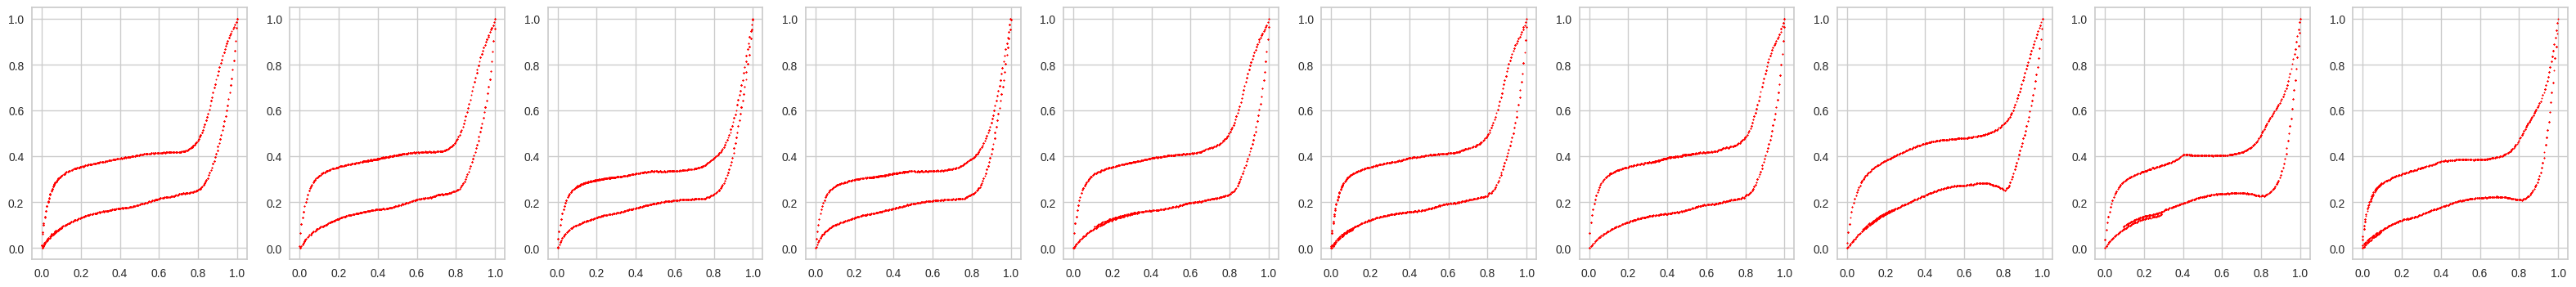
\includegraphics[width=1.0\textwidth]{figures/clusters/cv_cluster1.png}
Cluster 2:\\
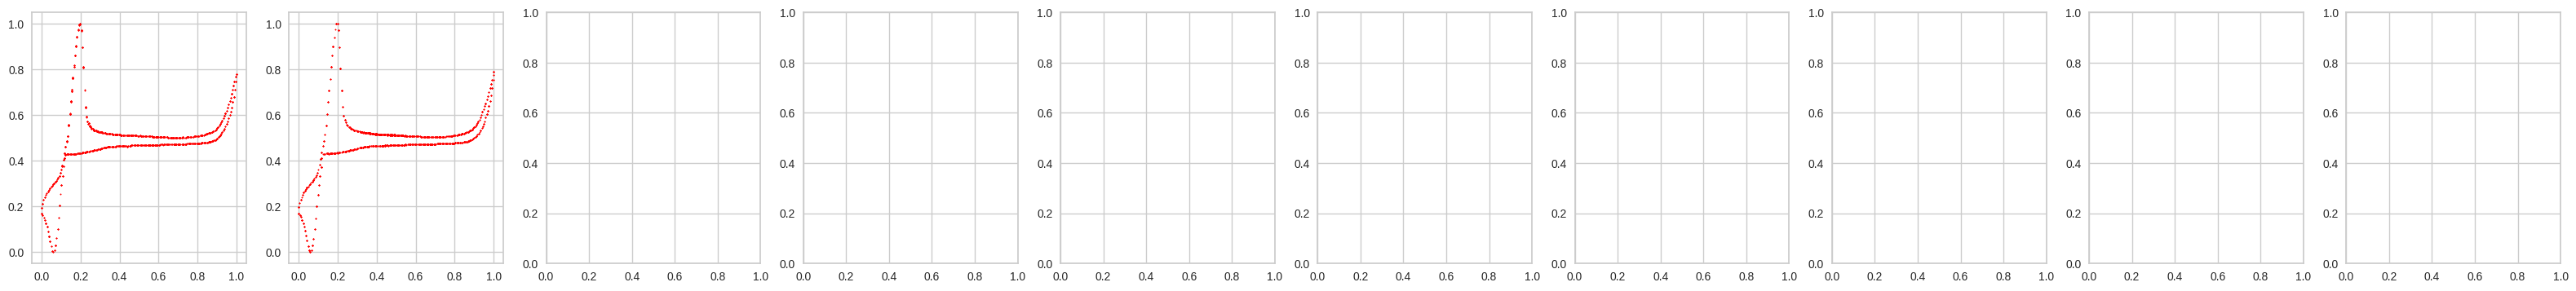
\includegraphics[width=1.0\textwidth]{figures/clusters/cv_cluster2.png}
Cluster 3:\\
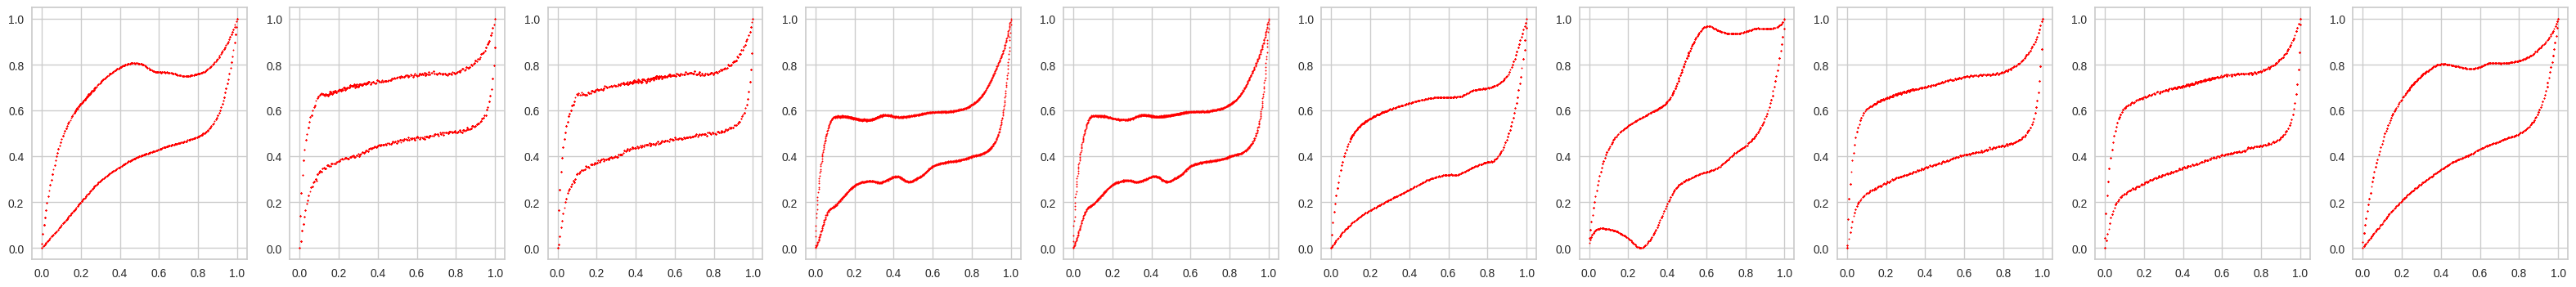
\includegraphics[width=1.0\textwidth]{figures/clusters/cv_cluster3.png}
Cluster 4:\\
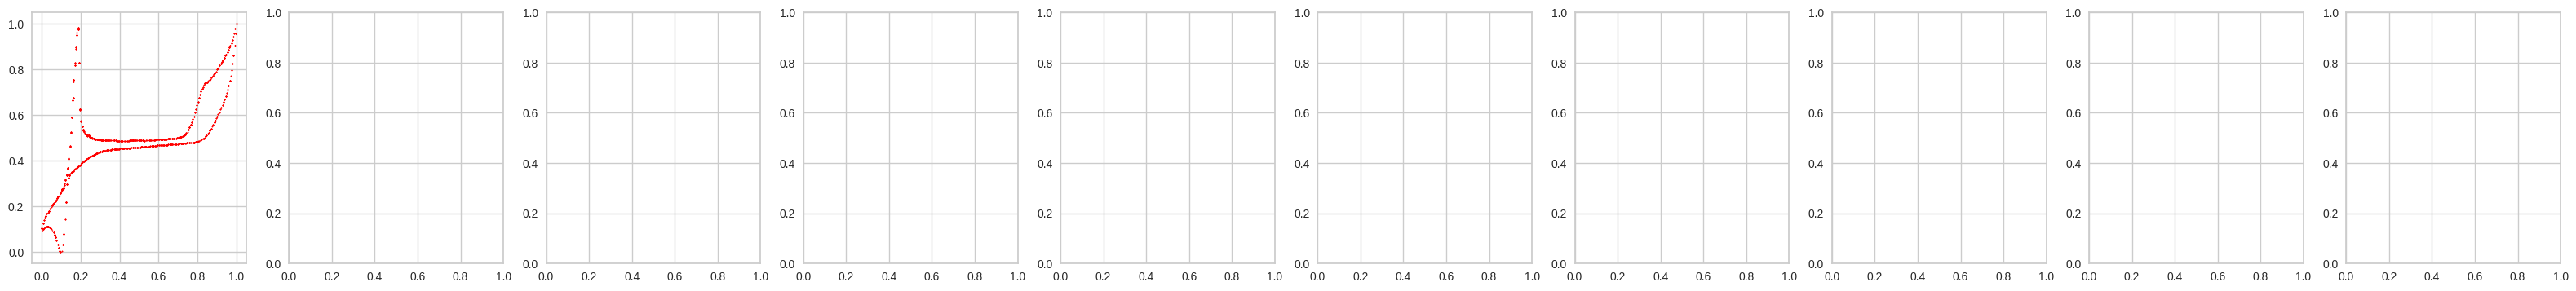
\includegraphics[width=1.0\textwidth]{figures/clusters/cv_cluster4.png}
Cluster 5:\\
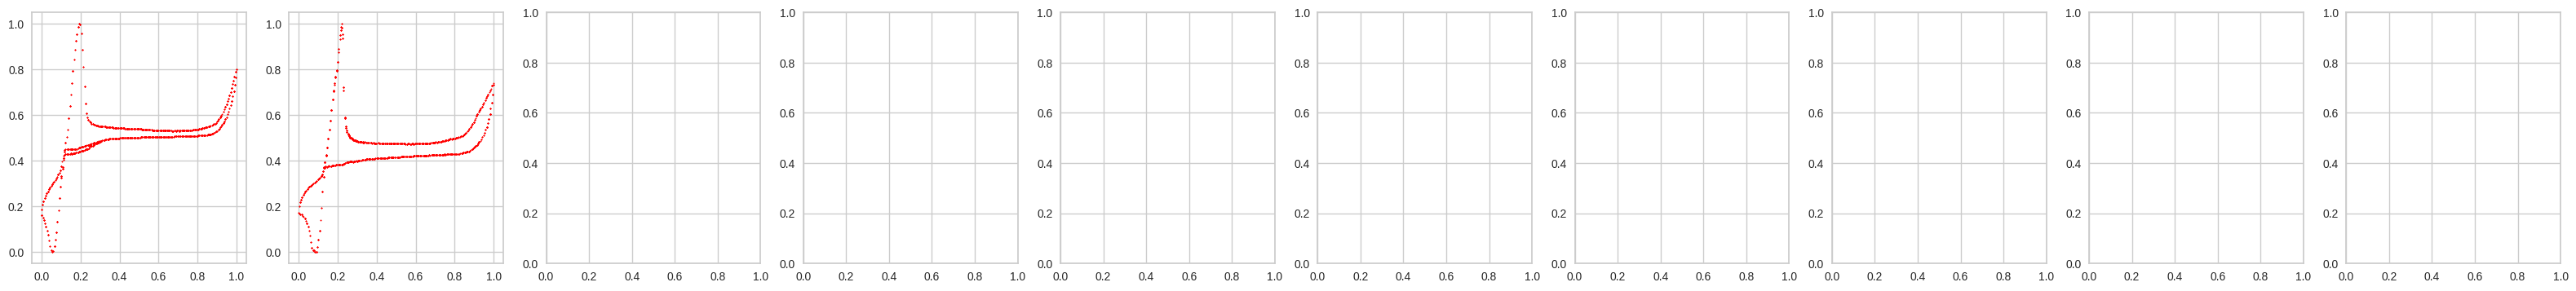
\includegraphics[width=1.0\textwidth]{figures/clusters/cv_cluster5.png}
Cluster 6:\\
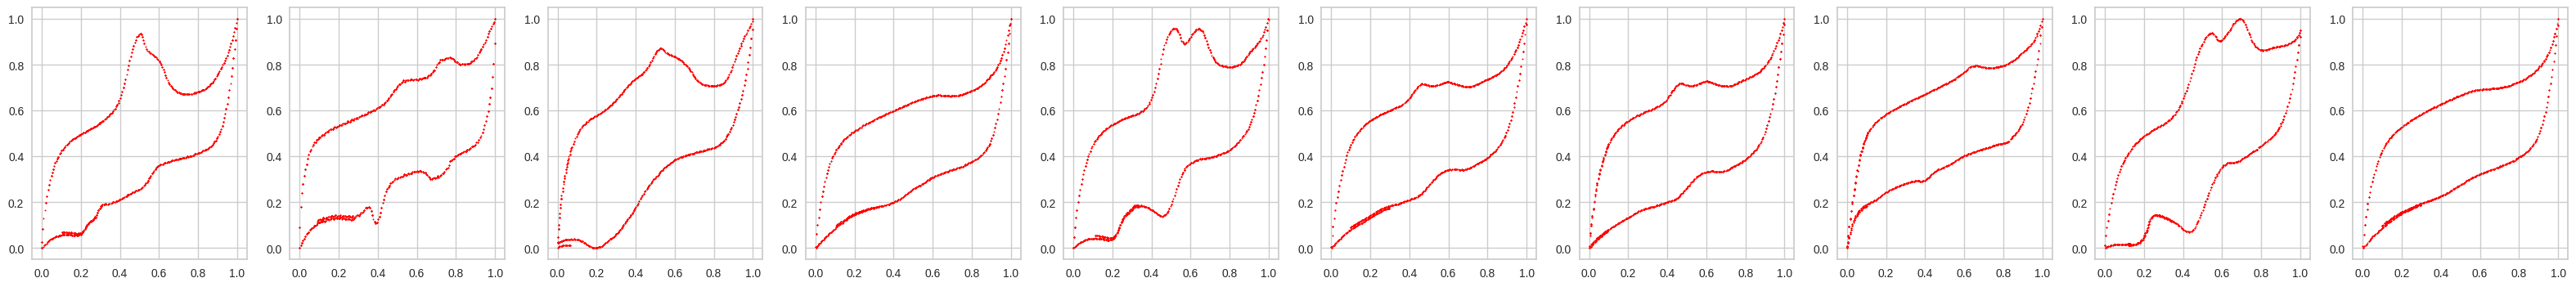
\includegraphics[width=1.0\textwidth]{figures/clusters/cv_cluster6.png}
Cluster 7:\\
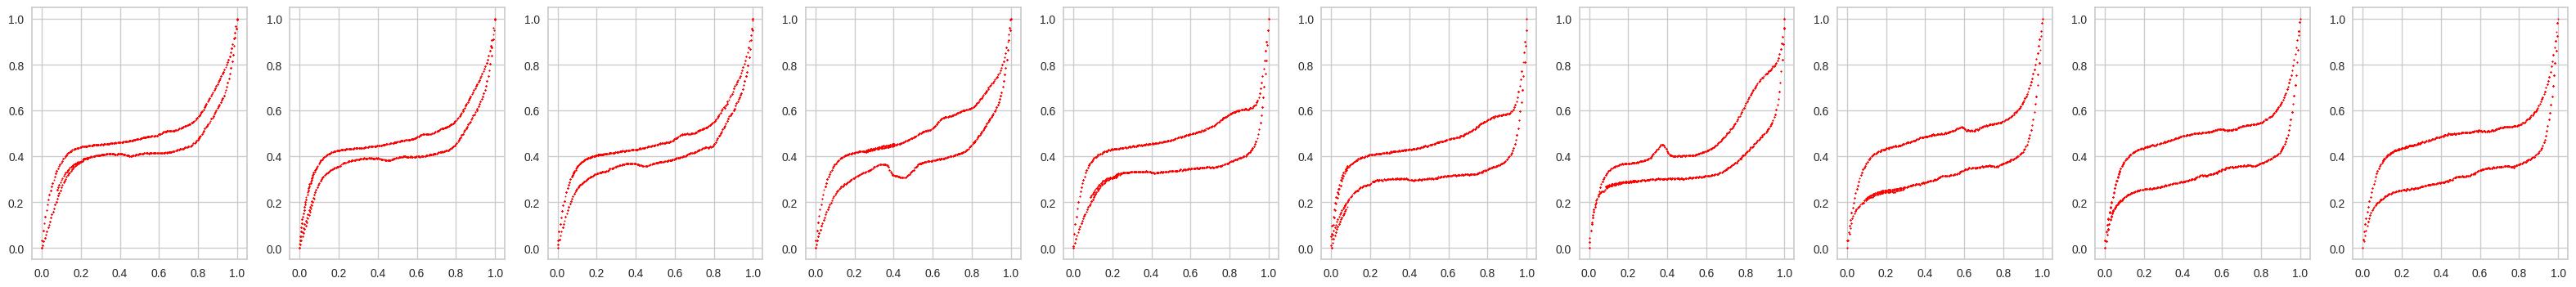
\includegraphics[width=1.0\textwidth]{figures/clusters/cv_cluster7.png}
Cluster 8:\\
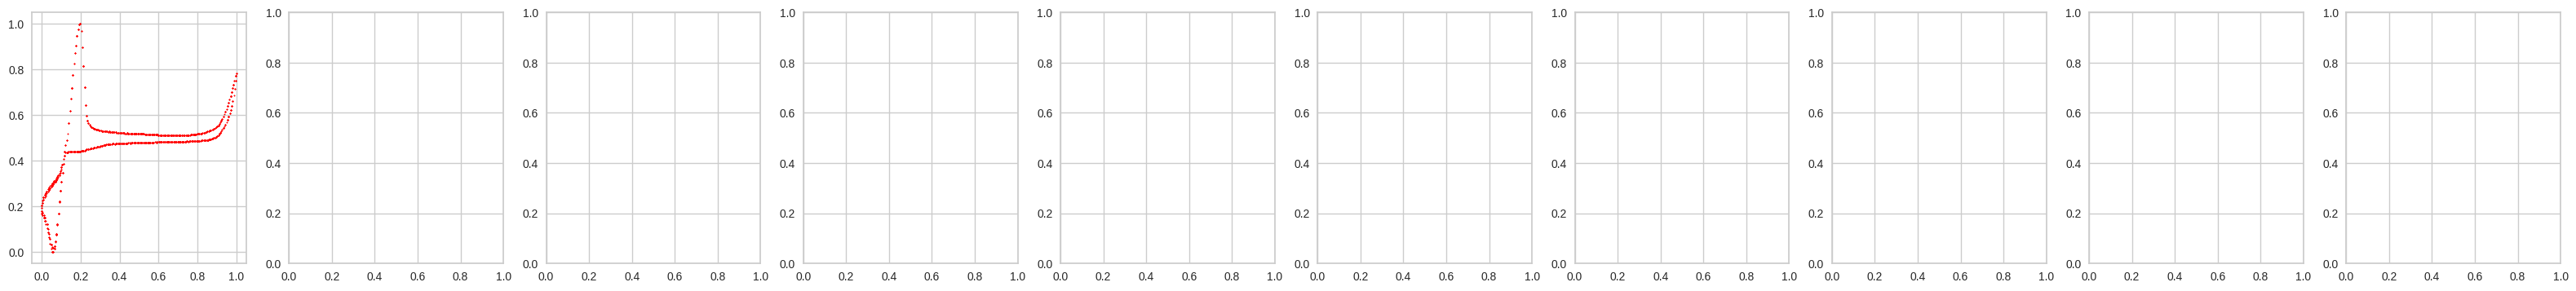
\includegraphics[width=1.0\textwidth]{figures/clusters/cv_cluster8.png}
Cluster 9:\\
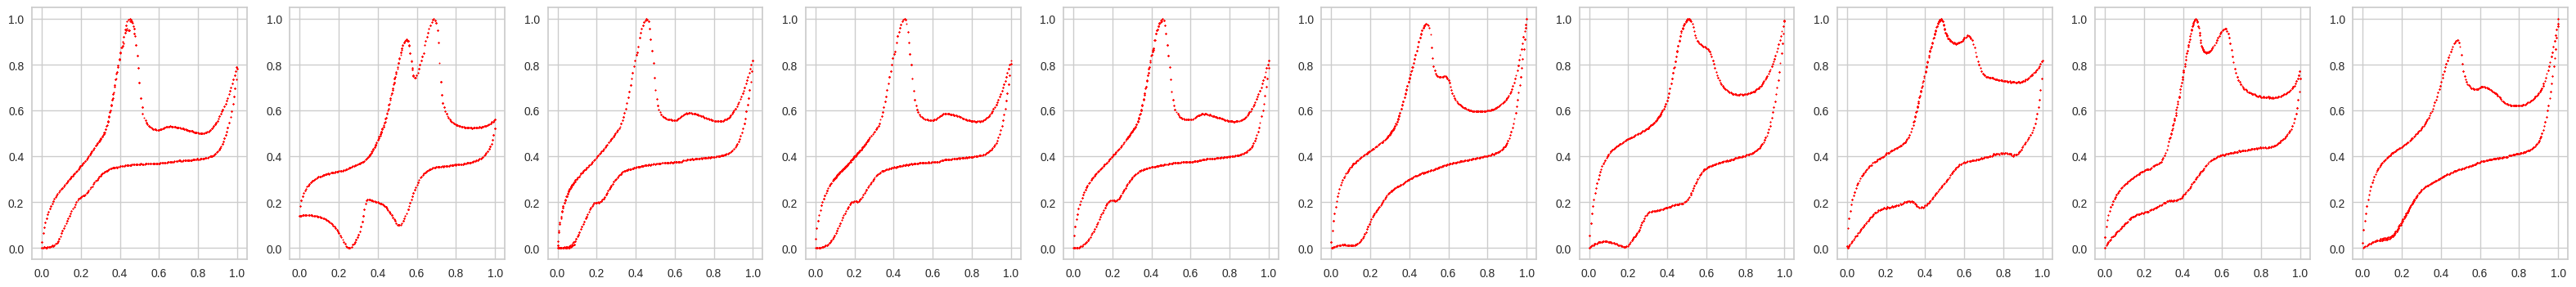
\includegraphics[width=1.0\textwidth]{figures/clusters/cv_cluster9.png}
Cluster 10:\\
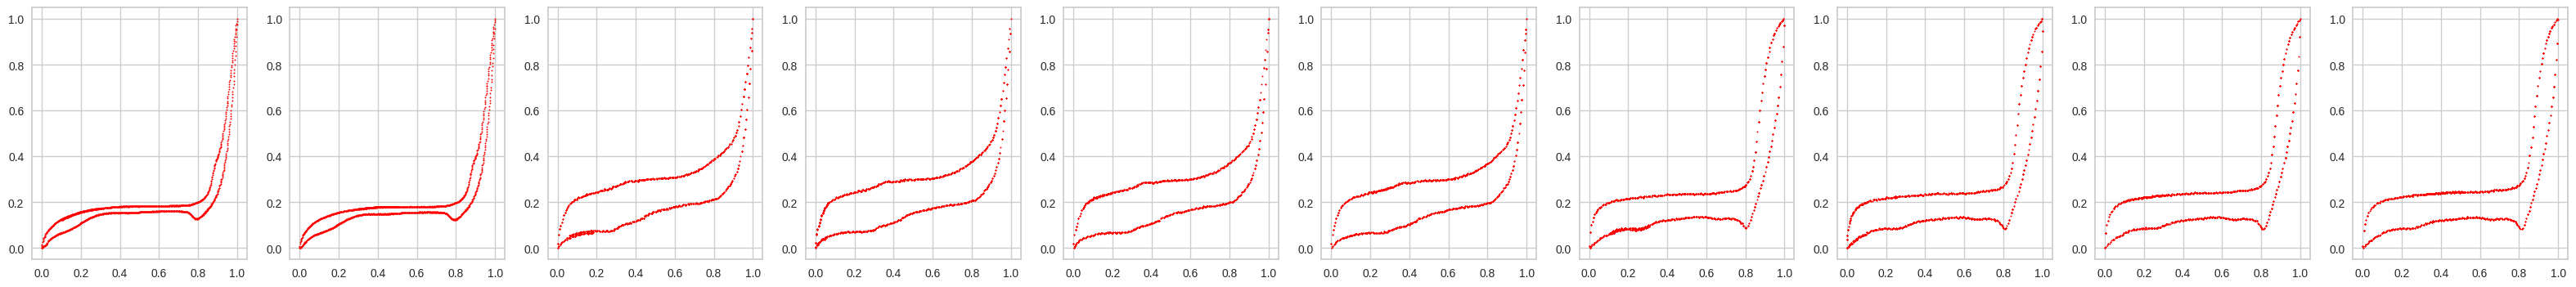
\includegraphics[width=1.0\textwidth]{figures/clusters/cv_cluster10.png}
Cluster 11:\\
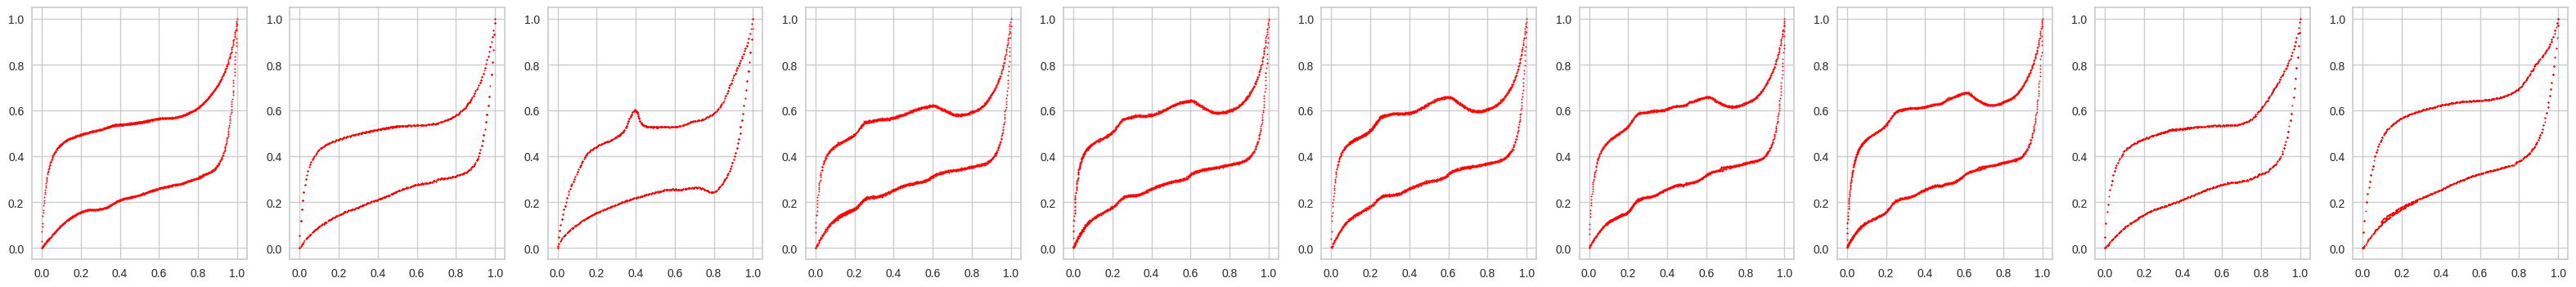
\includegraphics[width=1.0\textwidth]{figures/clusters/cv_cluster11.png}
Cluster 12:\\
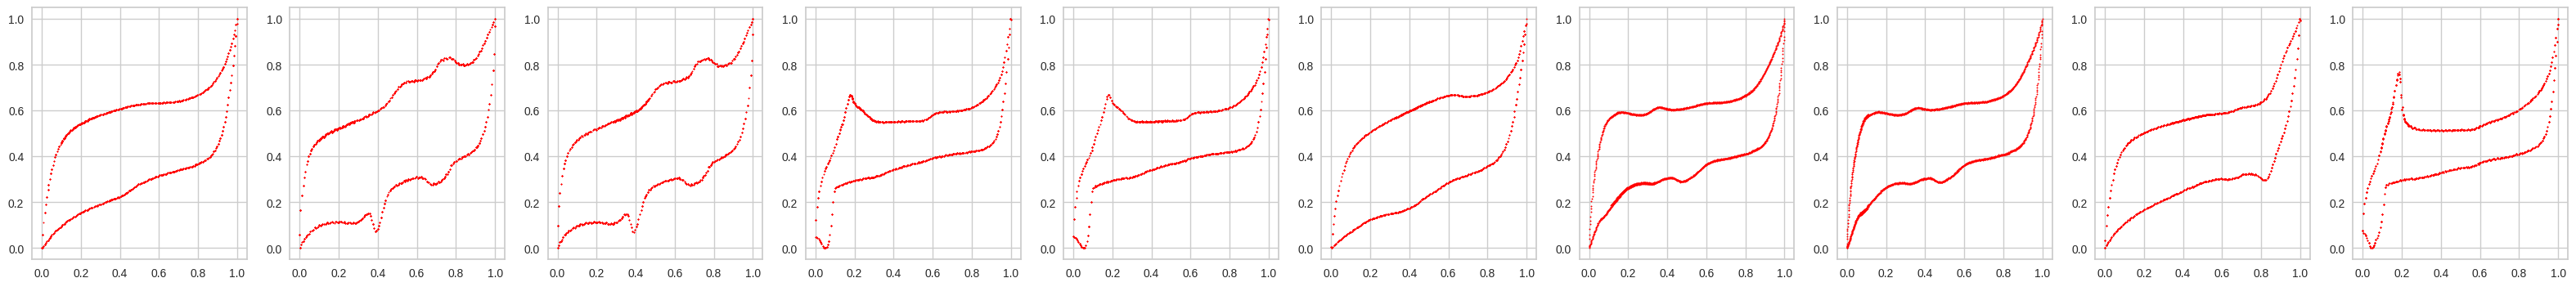
\includegraphics[width=1.0\textwidth]{figures/clusters/cv_cluster12.png}
Cluster 13:\\
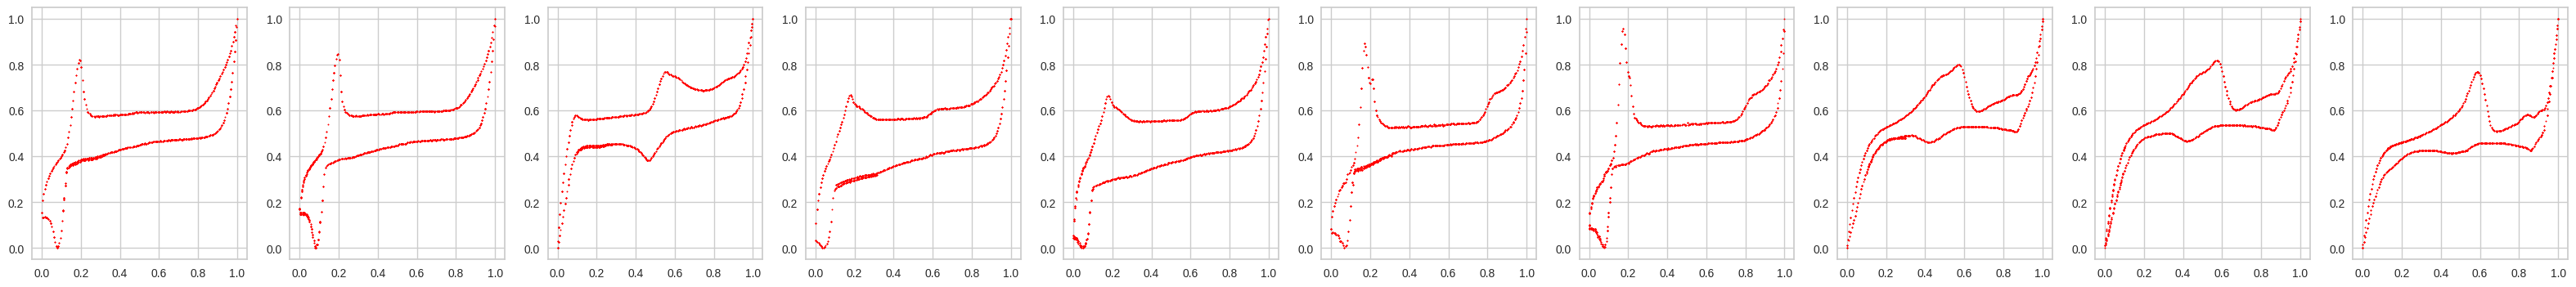
\includegraphics[width=1.0\textwidth]{figures/clusters/cv_cluster13.png}
Cluster 14:\\
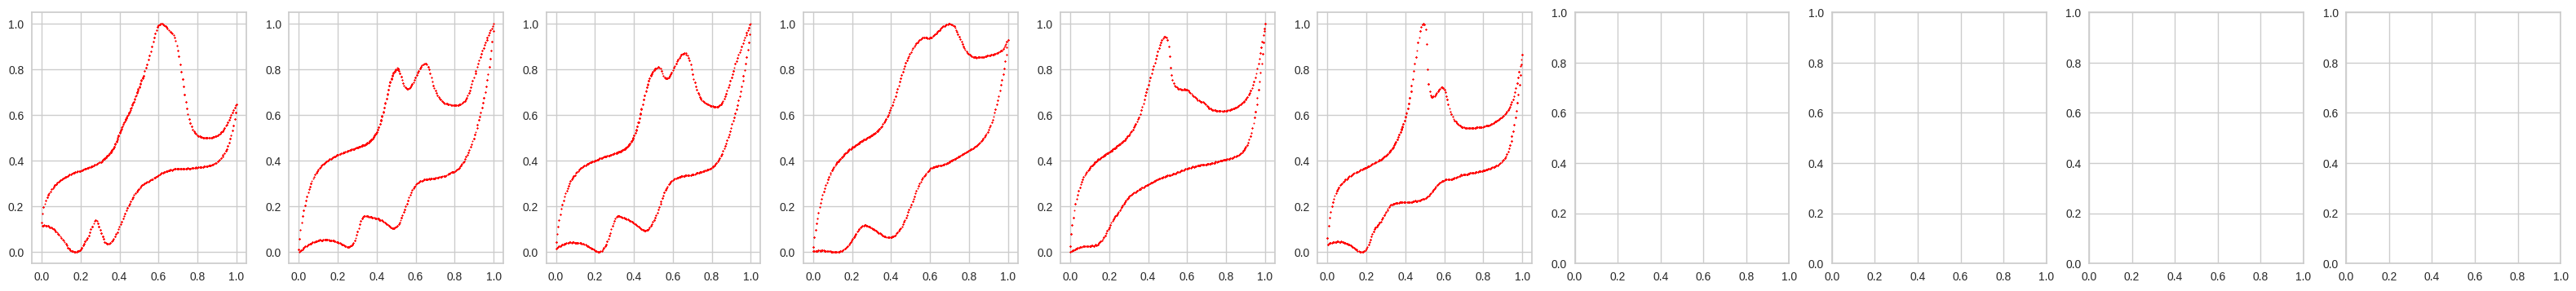
\includegraphics[width=1.0\textwidth]{figures/clusters/cv_cluster14.png}
Cluster 15:\\
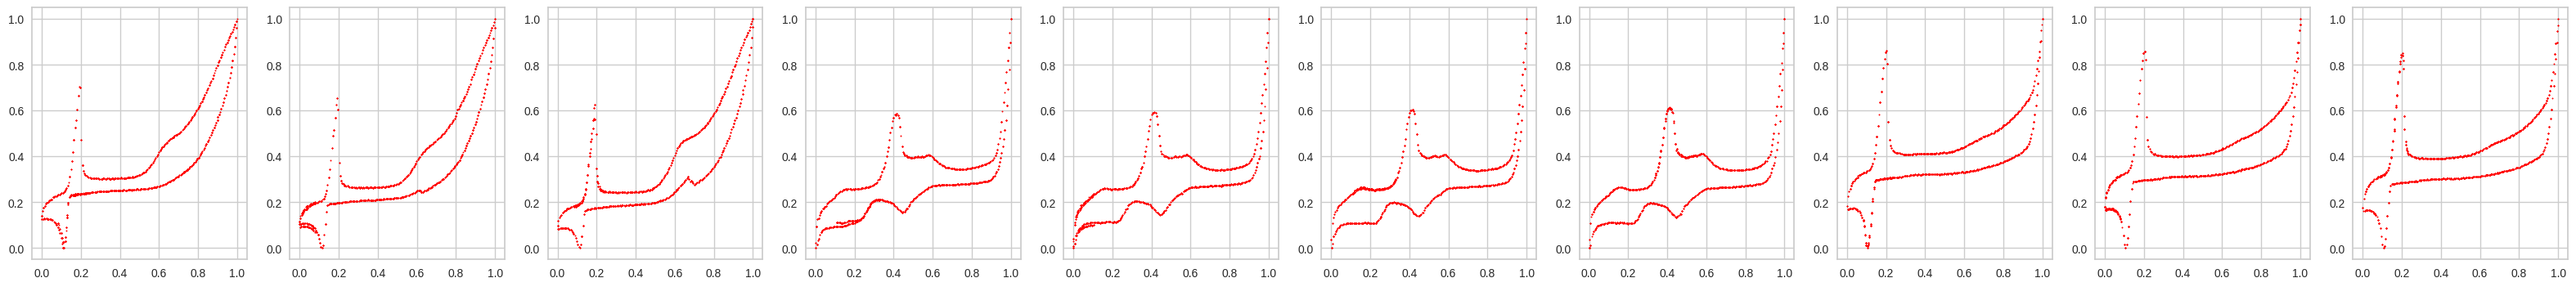
\includegraphics[width=1.0\textwidth]{figures/clusters/cv_cluster15.png}
Cluster 16:\\
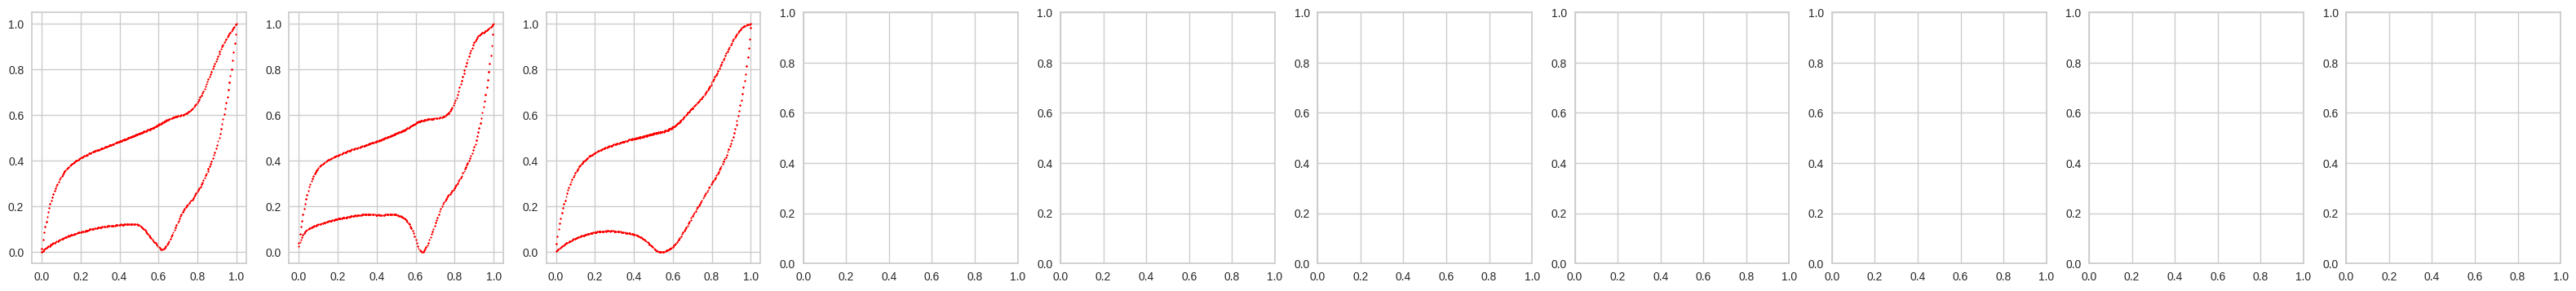
\includegraphics[width=1.0\textwidth]{figures/clusters/cv_cluster16.png}
Cluster 17:\\
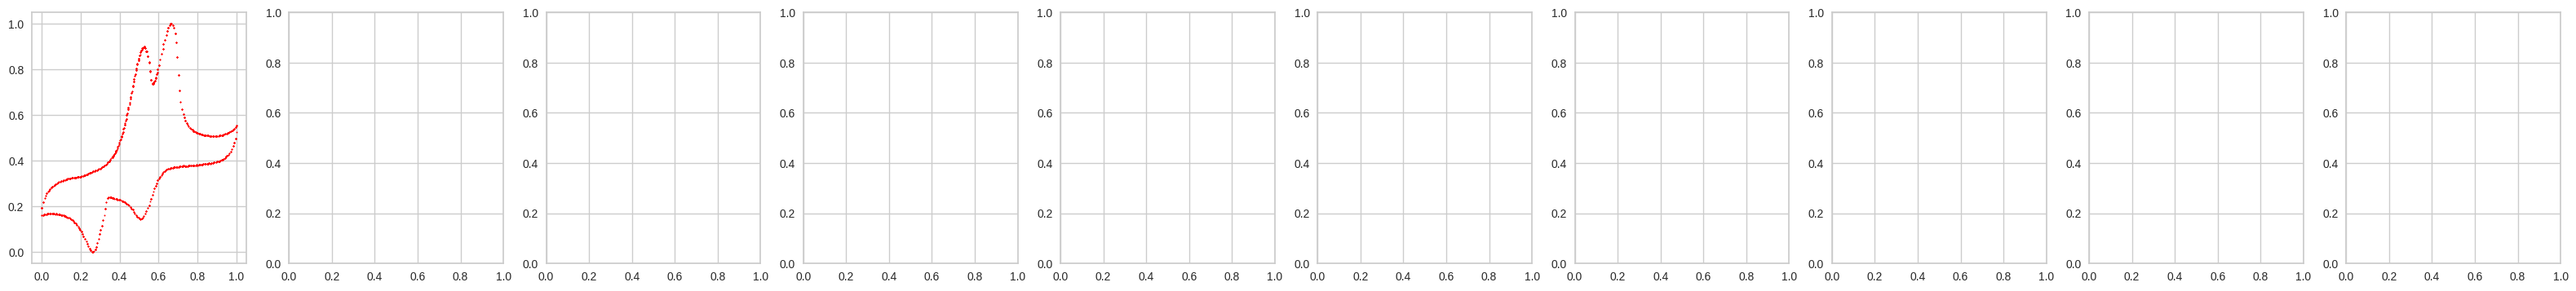
\includegraphics[width=1.0\textwidth]{figures/clusters/cv_cluster17.png}
Cluster 18:\\
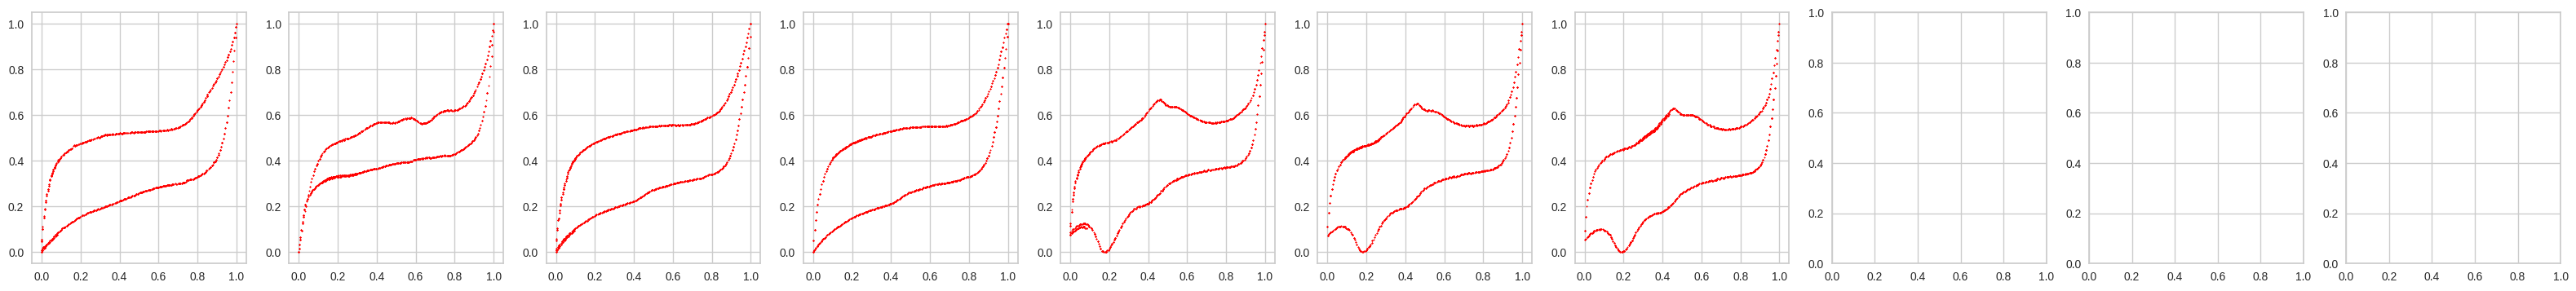
\includegraphics[width=1.0\textwidth]{figures/clusters/cv_cluster18.png}
Cluster 19:\\
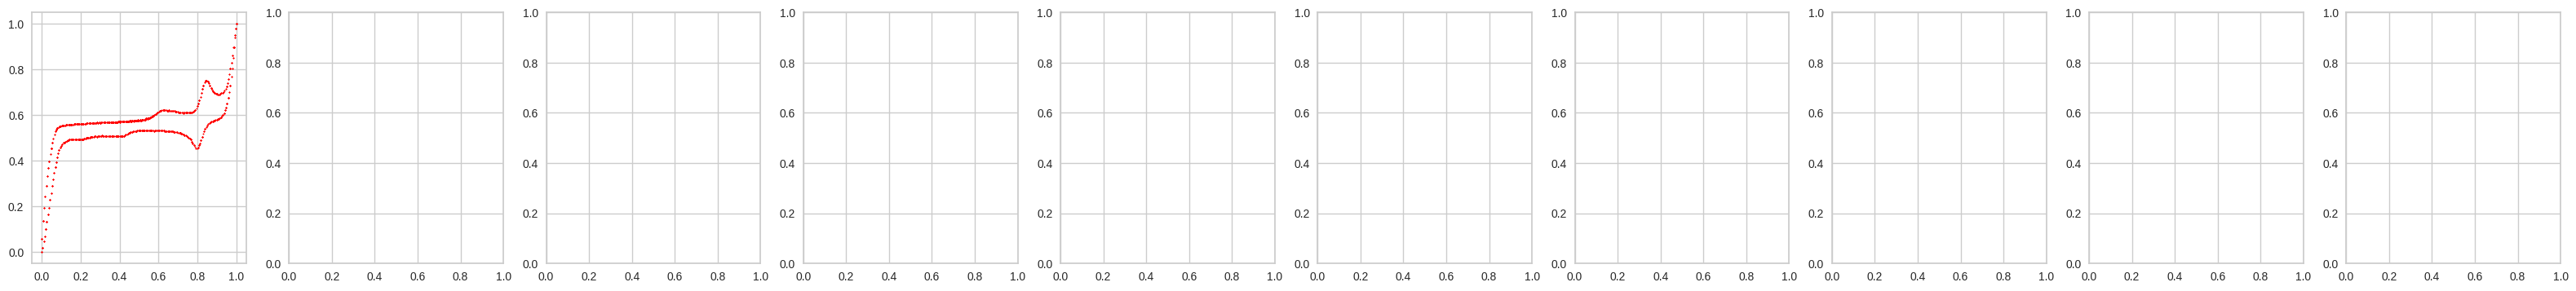
\includegraphics[width=1.0\textwidth]{figures/clusters/cv_cluster19.png}
Cluster 20:\\
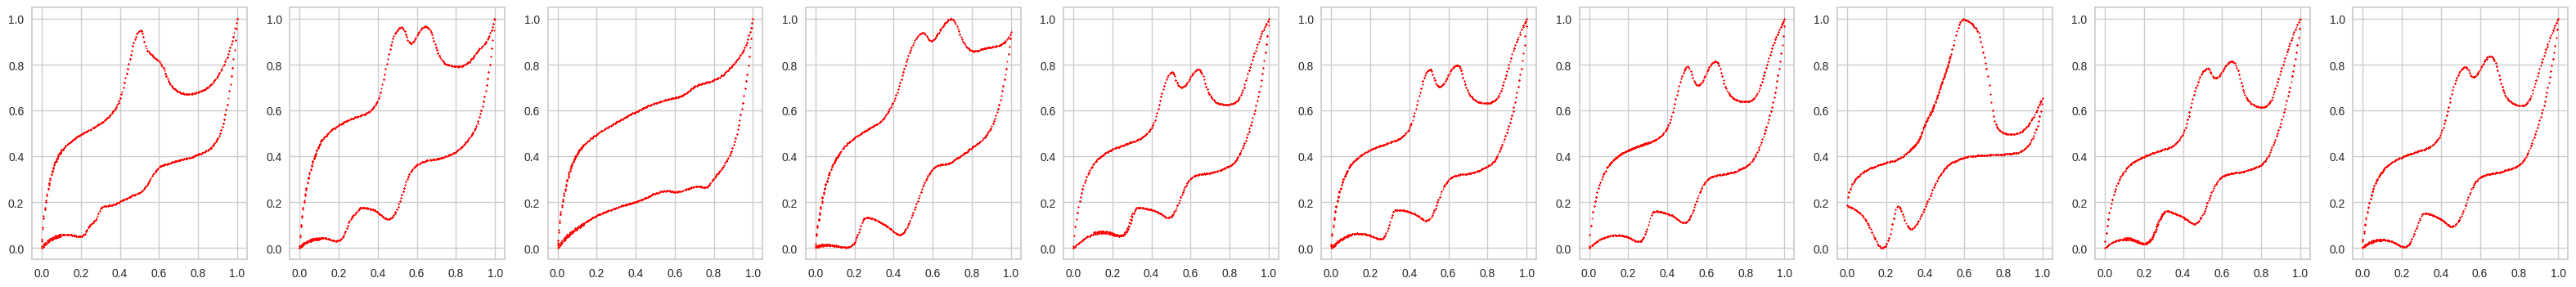
\includegraphics[width=1.0\textwidth]{figures/clusters/cv_cluster20.png}
Cluster 21:\\
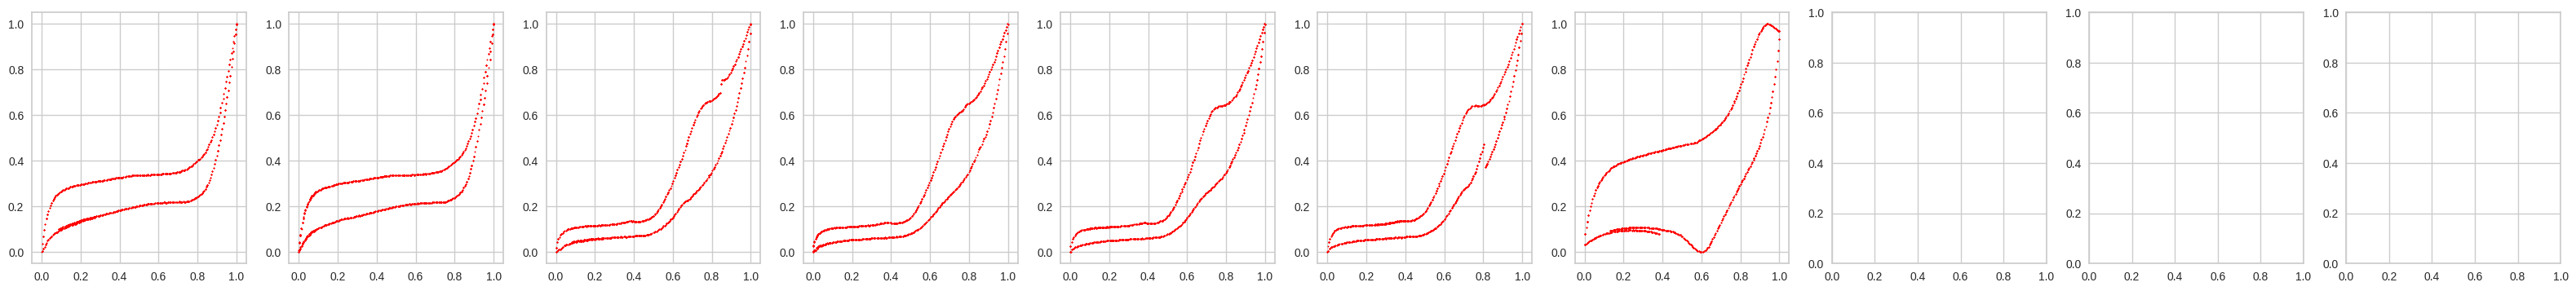
\includegraphics[width=1.0\textwidth]{figures/clusters/cv_cluster21.png}
Cluster 22:\\
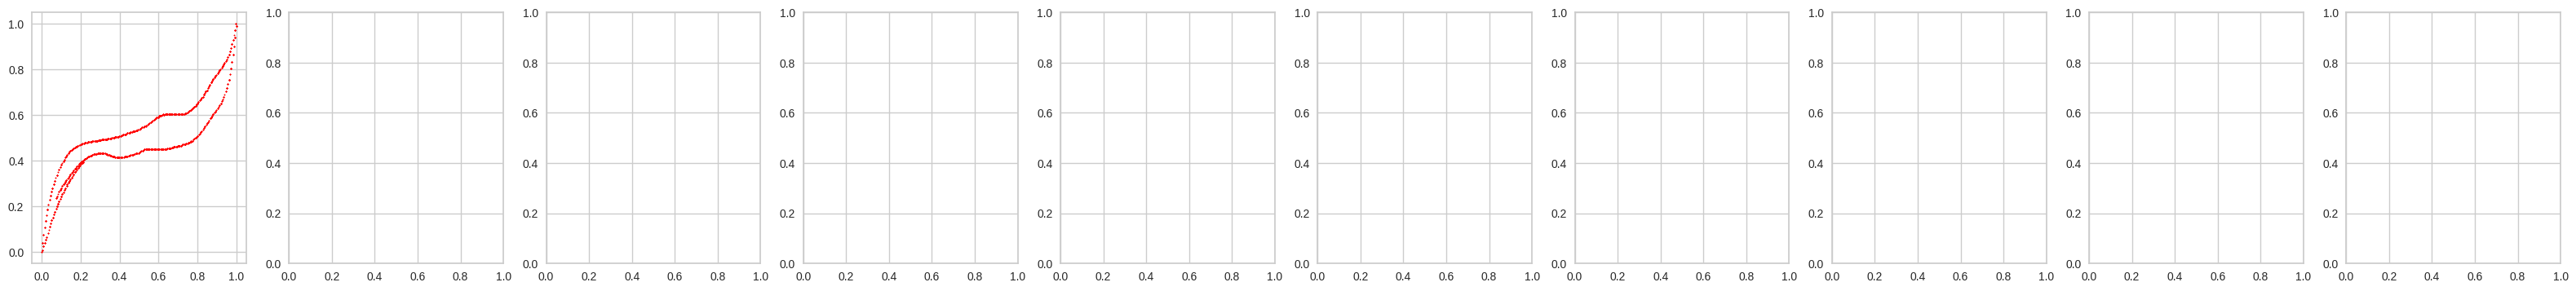
\includegraphics[width=1.0\textwidth]{figures/clusters/cv_cluster22.png}
Cluster 23:\\
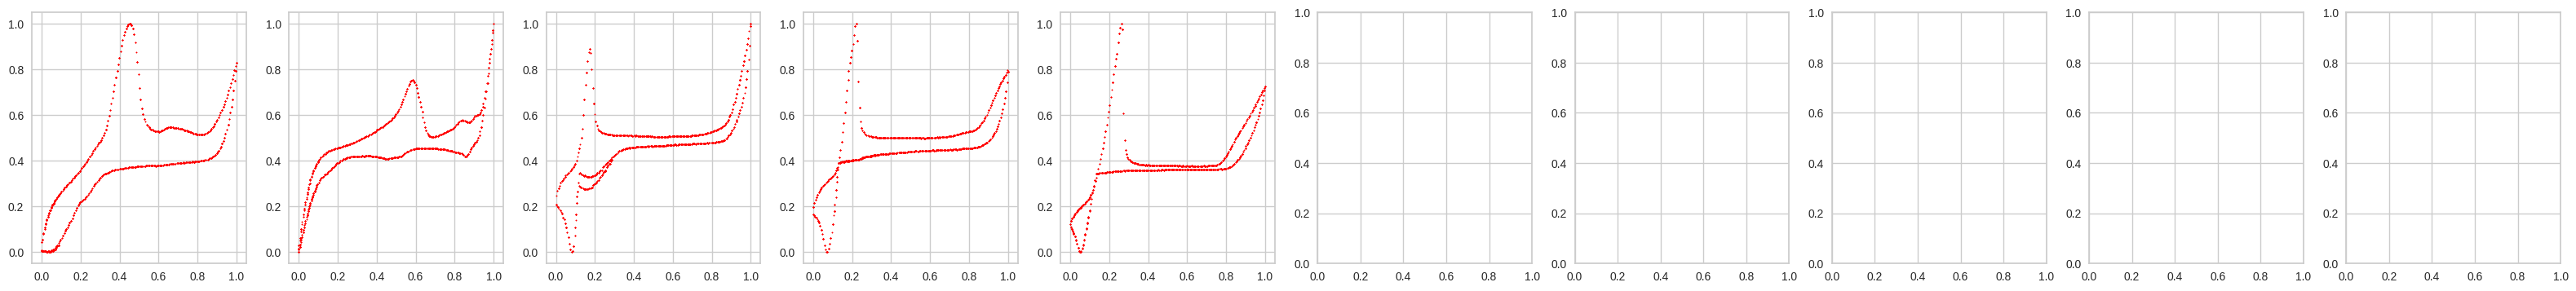
\includegraphics[width=1.0\textwidth]{figures/clusters/cv_cluster23.png}
Cluster 24:\\
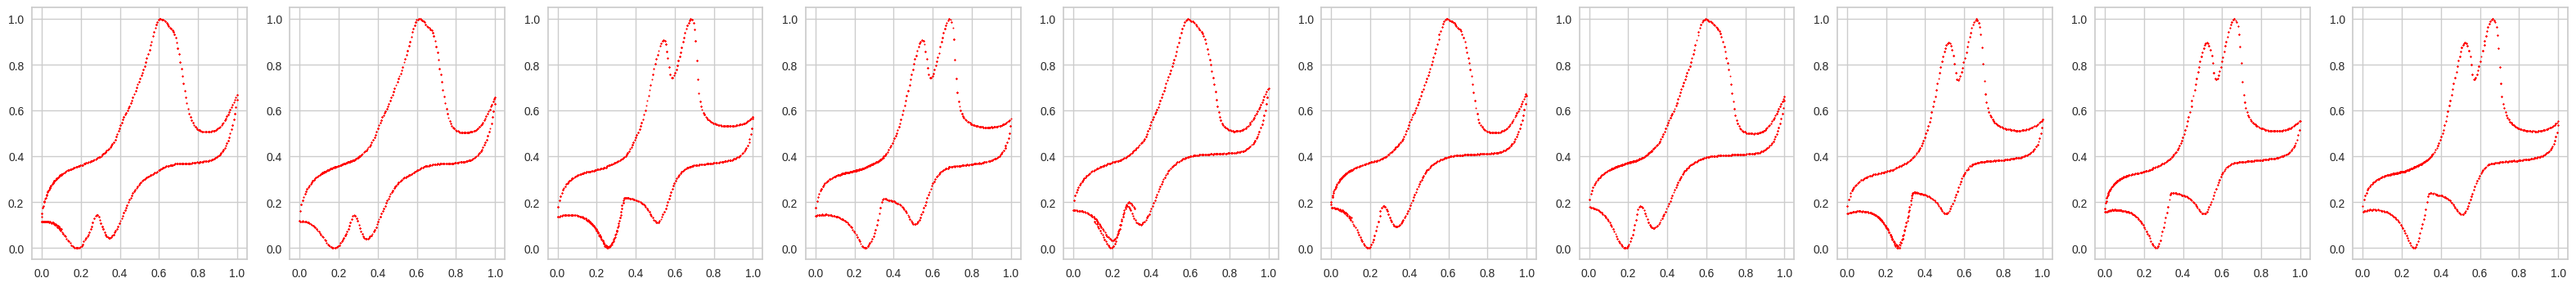
\includegraphics[width=1.0\textwidth]{figures/clusters/cv_cluster24.png}
Cluster 25:\\
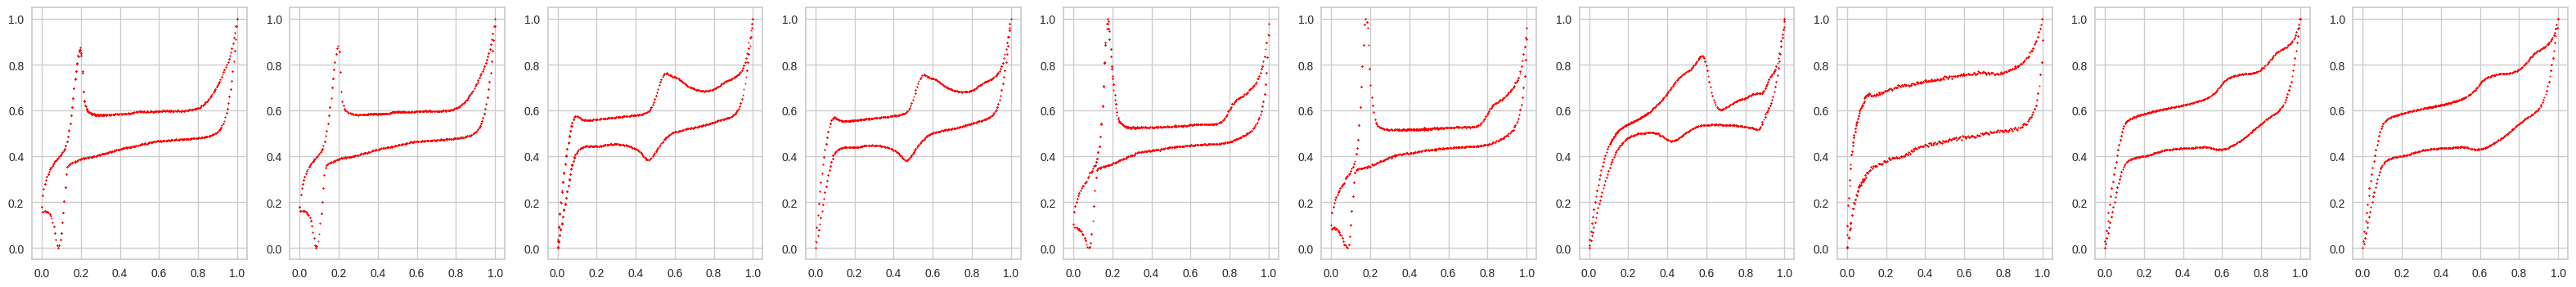
\includegraphics[width=1.0\textwidth]{figures/clusters/cv_cluster25.png}
Cluster 26:\\
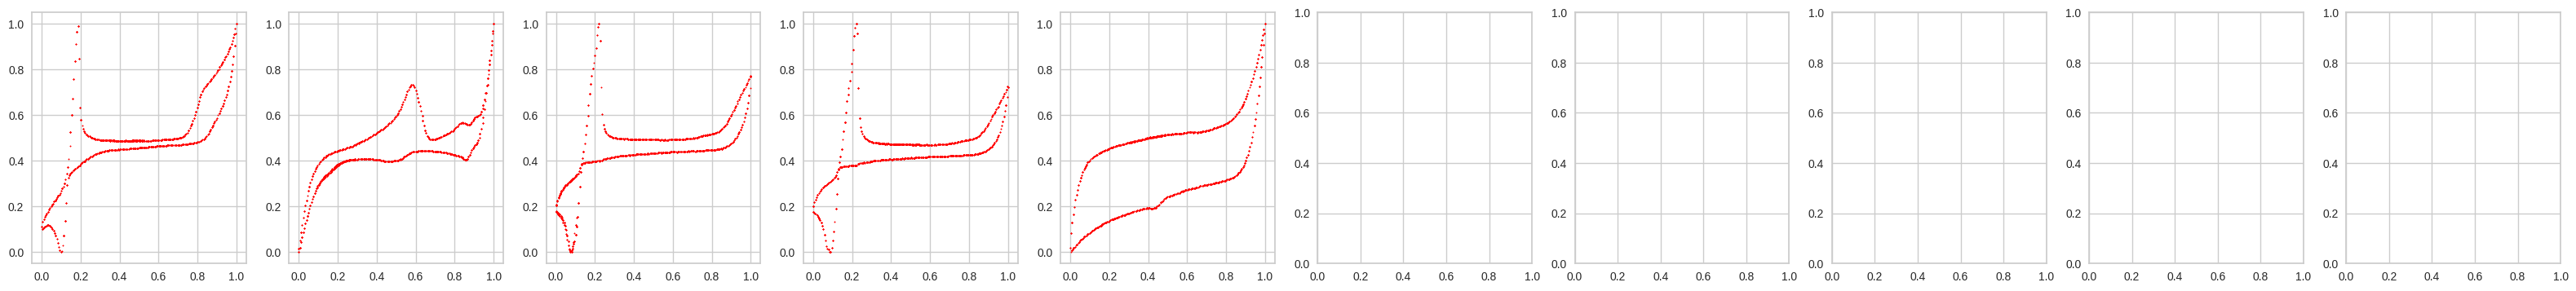
\includegraphics[width=1.0\textwidth]{figures/clusters/cv_cluster26.png}
Cluster 27:\\
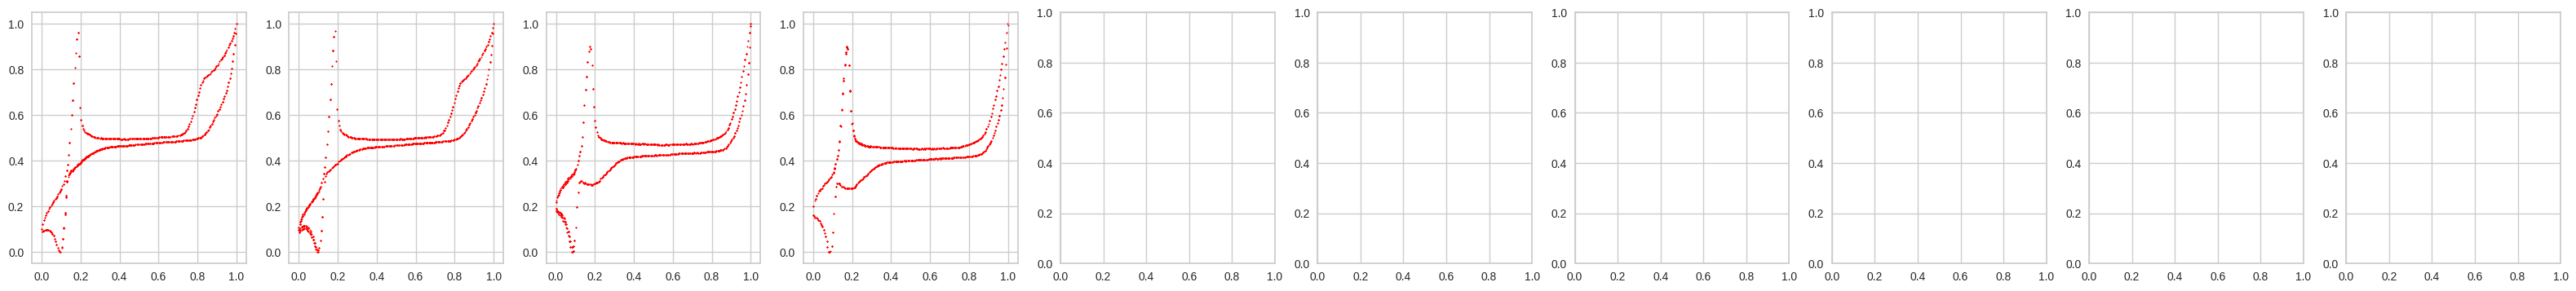
\includegraphics[width=1.0\textwidth]{figures/clusters/cv_cluster27.png}
Cluster 28:\\
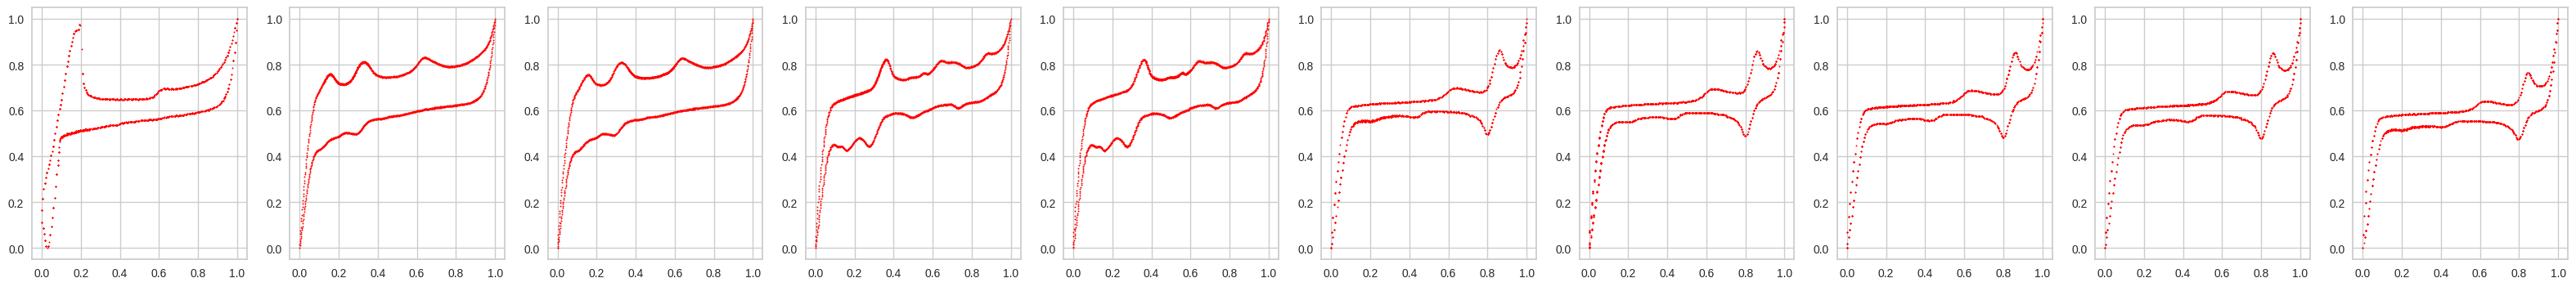
\includegraphics[width=1.0\textwidth]{figures/clusters/cv_cluster28.png}
Cluster 29:\\
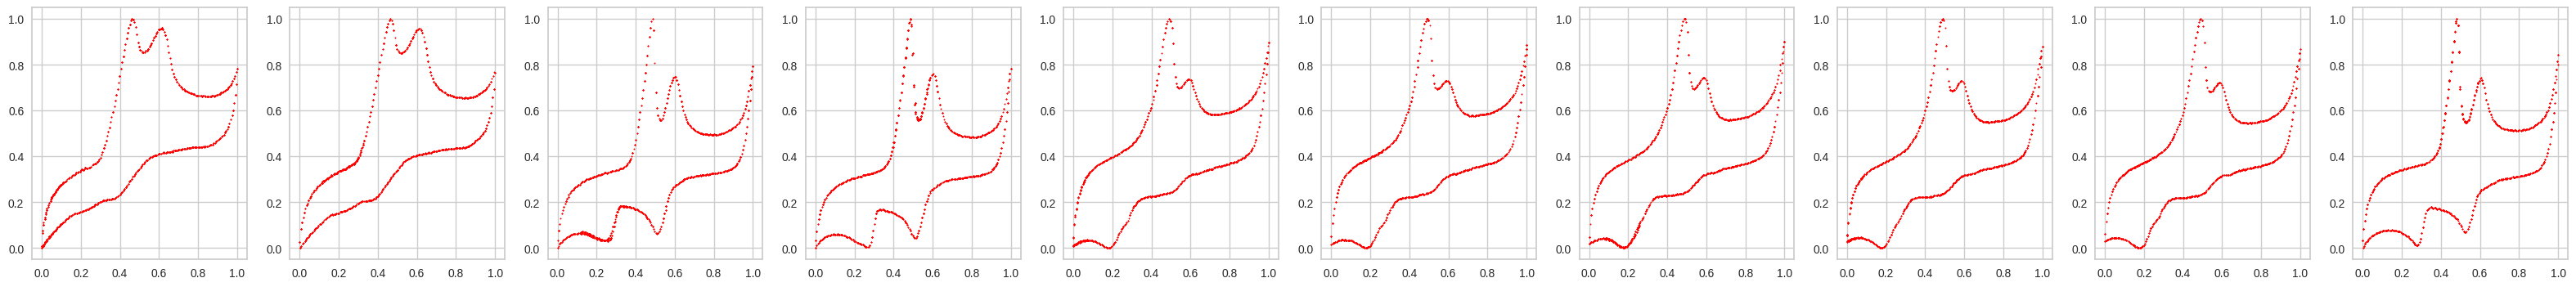
\includegraphics[width=1.0\textwidth]{figures/clusters/cv_cluster29.png}
Cluster 30:\\
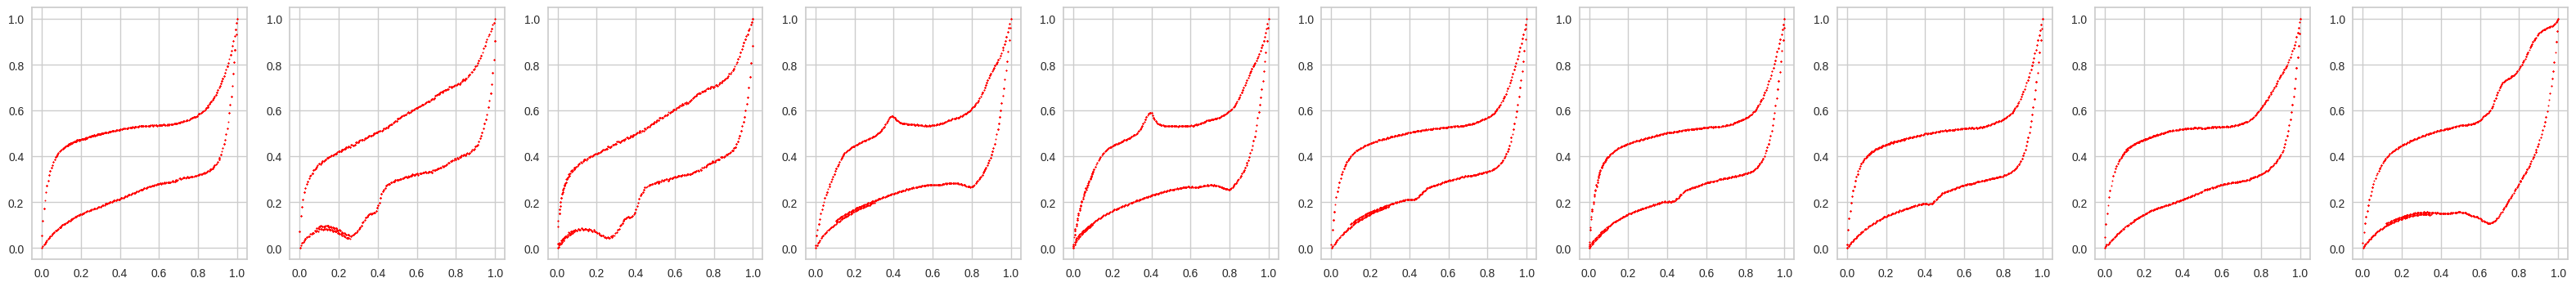
\includegraphics[width=1.0\textwidth]{figures/clusters/cv_cluster30.png}
Cluster 31:\\
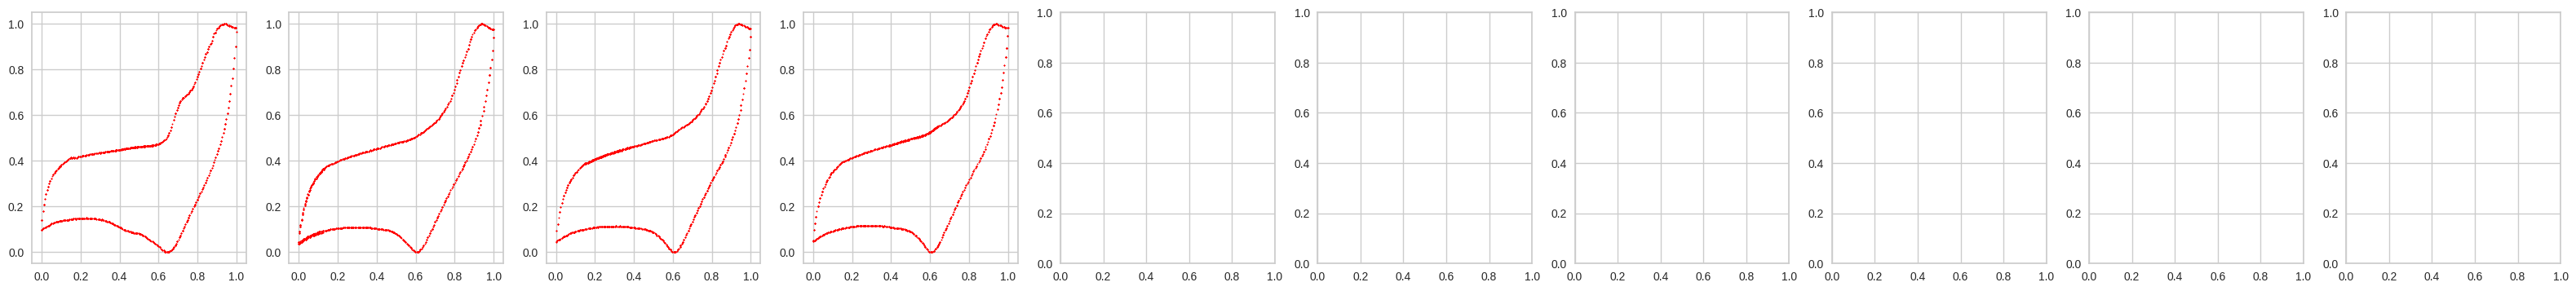
\includegraphics[width=1.0\textwidth]{figures/clusters/cv_cluster31.png}
Cluster 32:\\
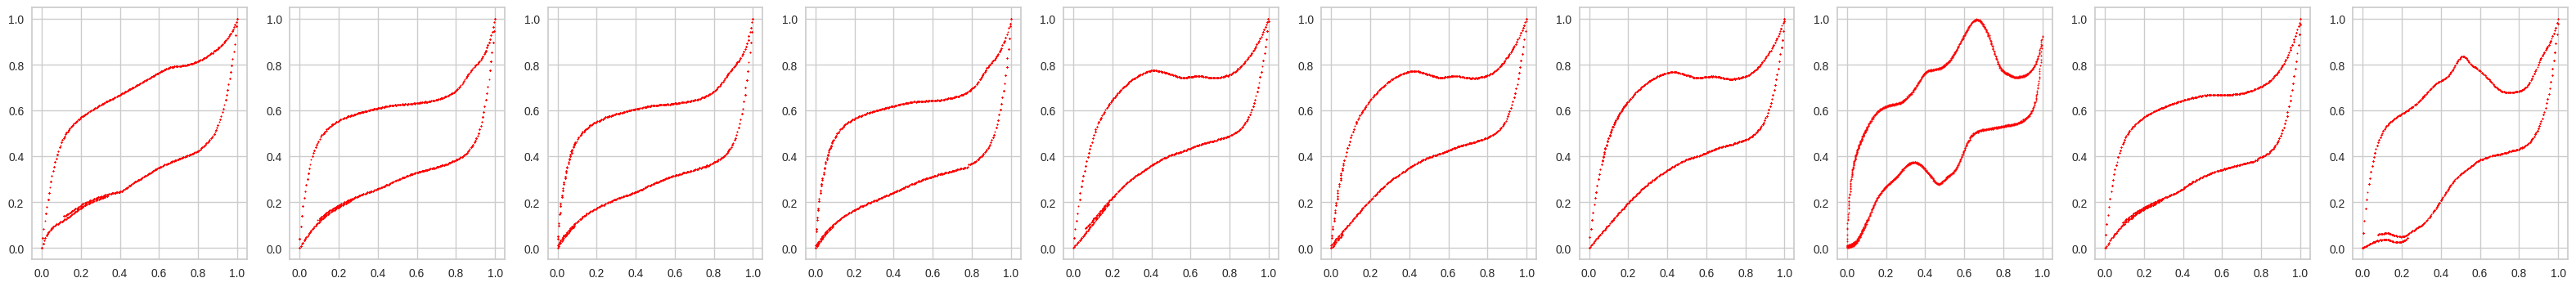
\includegraphics[width=1.0\textwidth]{figures/clusters/cv_cluster32.png}
Cluster 33:\\
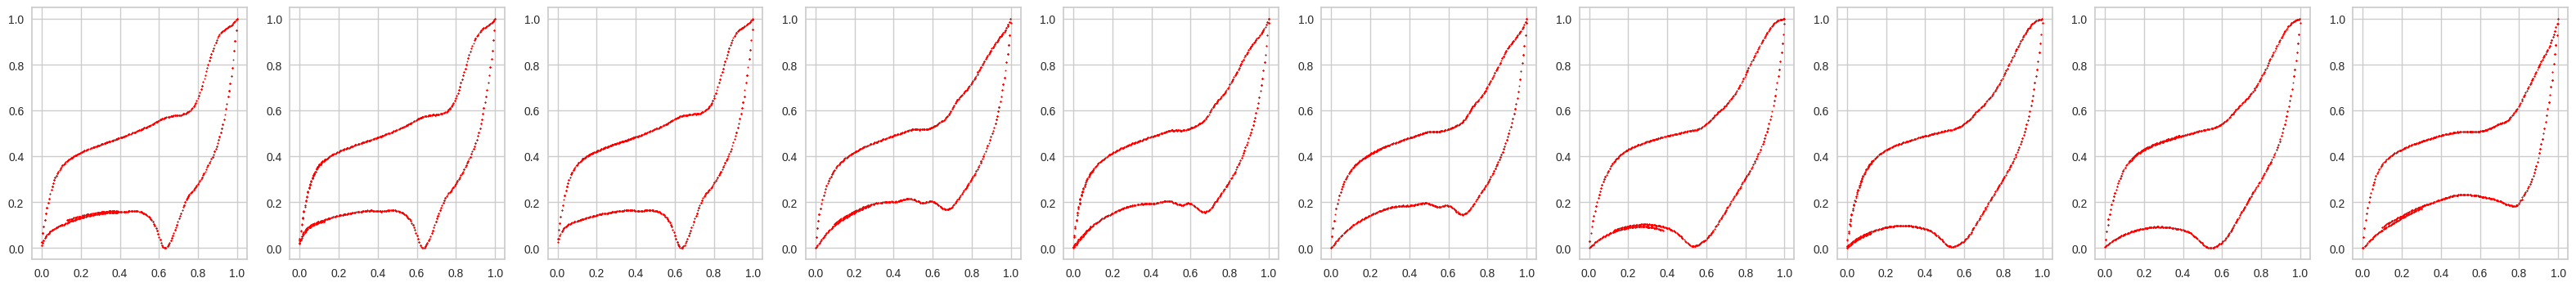
\includegraphics[width=1.0\textwidth]{figures/clusters/cv_cluster33.png}
Cluster 34:\\
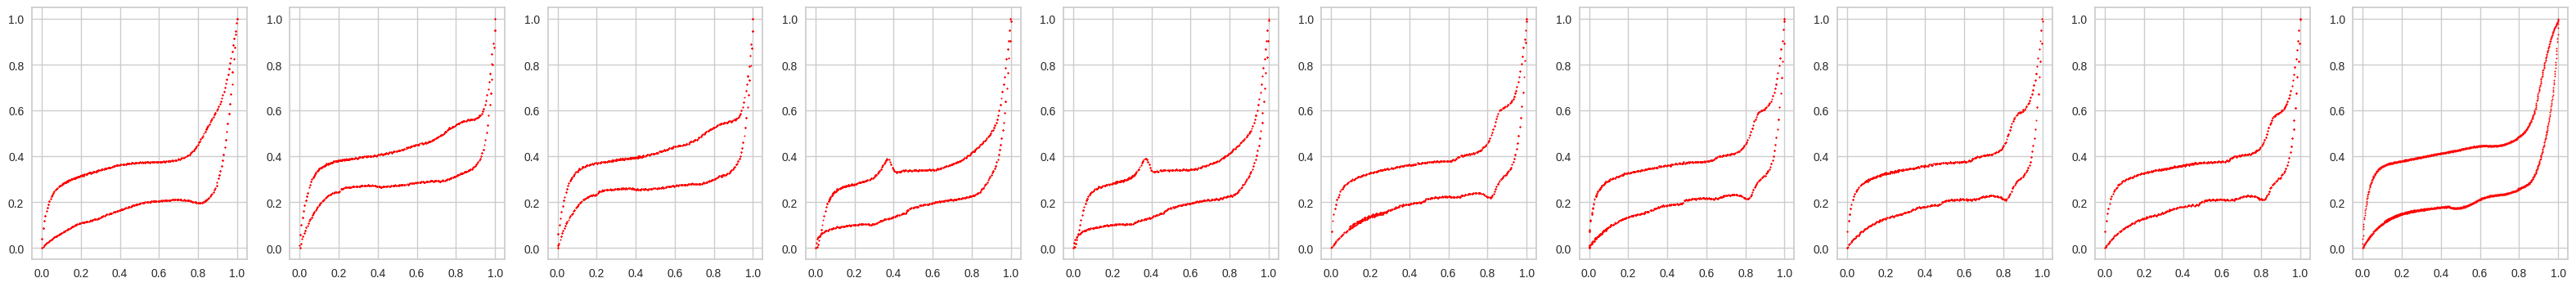
\includegraphics[width=1.0\textwidth]{figures/clusters/cv_cluster34.png}
Cluster 35:\\
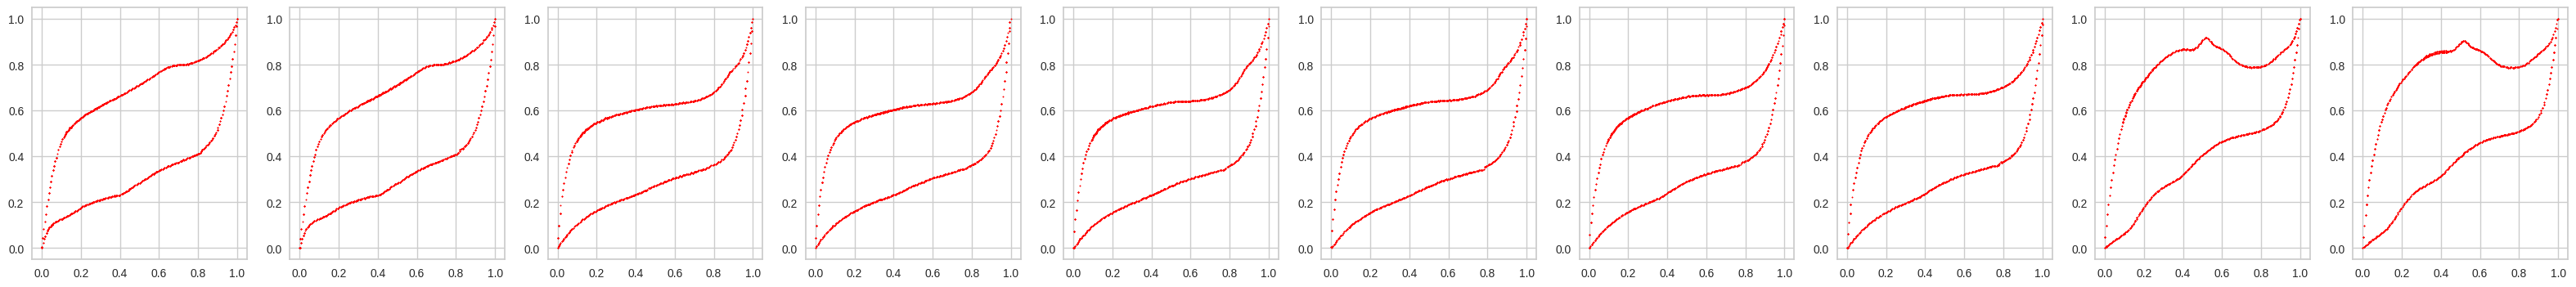
\includegraphics[width=1.0\textwidth]{figures/clusters/cv_cluster35.png}
Cluster 36:\\
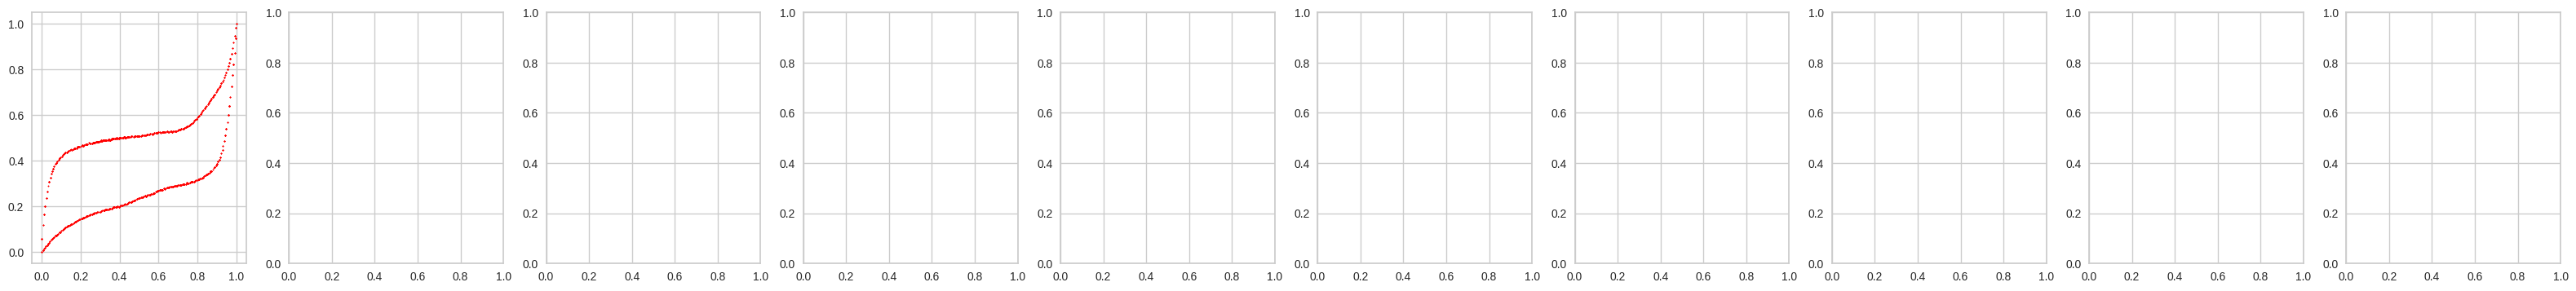
\includegraphics[width=1.0\textwidth]{figures/clusters/cv_cluster36.png}
Cluster 37:\\
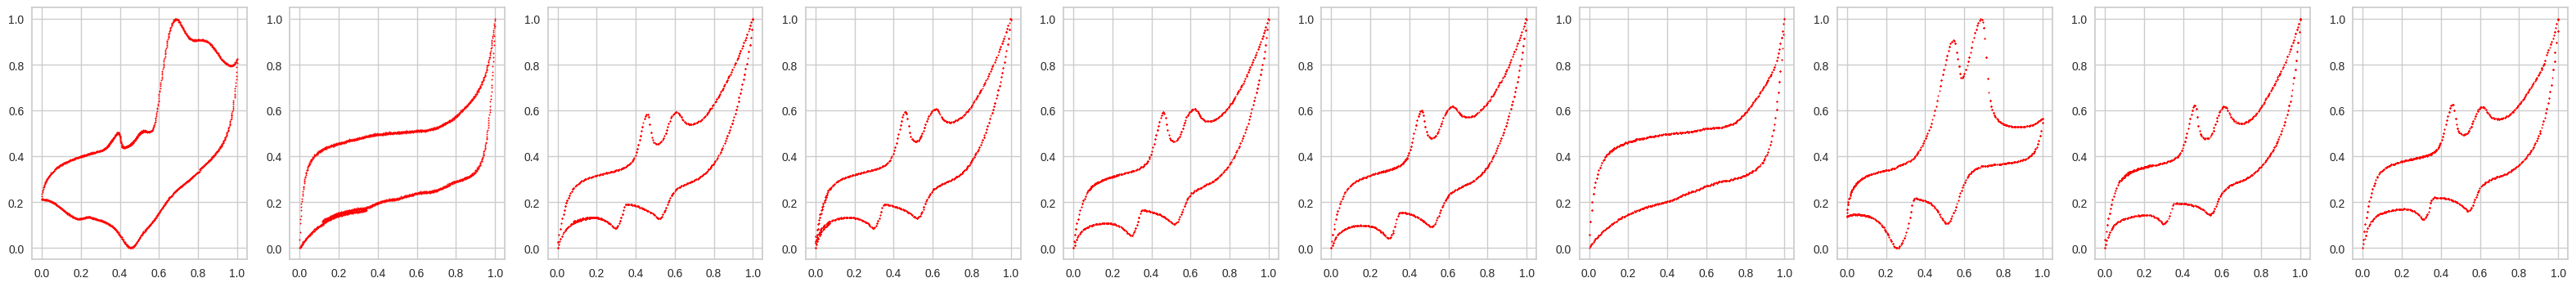
\includegraphics[width=1.0\textwidth]{figures/clusters/cv_cluster37.png}
Cluster 38:\\
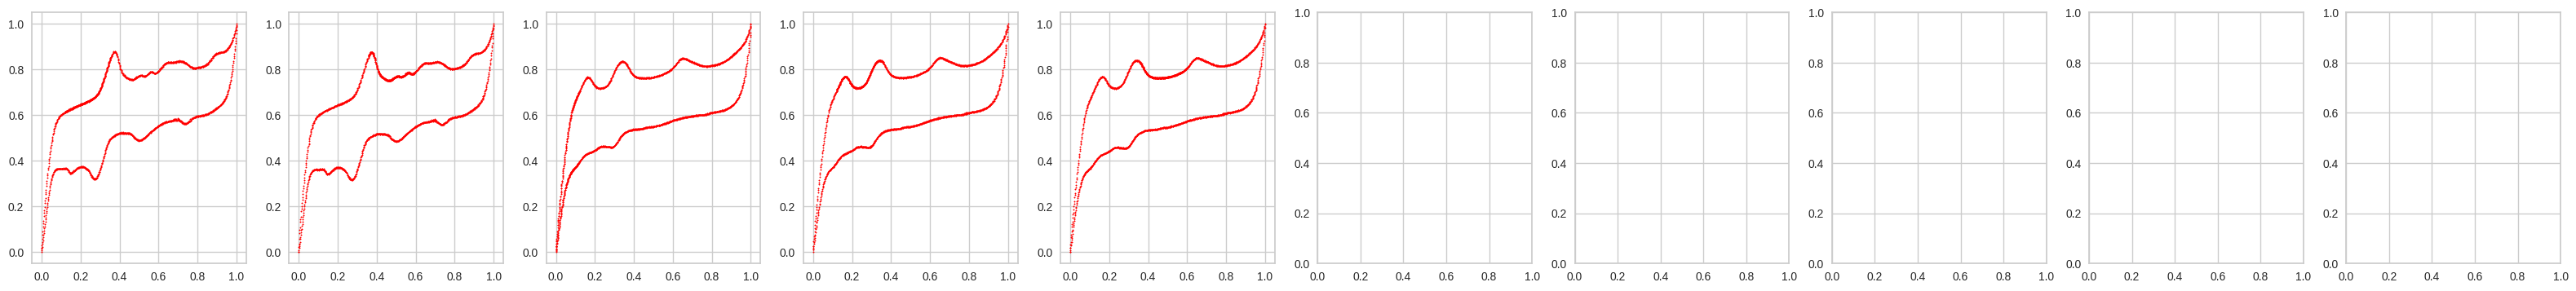
\includegraphics[width=1.0\textwidth]{figures/clusters/cv_cluster38.png}

\section{Metals and Ligands}
\begin{table}[!h]
\begin{center}
\begin{tabular}{c|c|c|c}
Entry & Metal & Form & CAS \\
\hline
1 & V(IV) & $\mathrm{VOSO_4 xH_2O}$ & 123334-20-3\\
2 & Cr(III) & $\mathrm{CrK(SO_4)_2 12H_2O}$ & 7788-99-0\\
3 & Mn(II) & $\mathrm{MnSO_4H_2O}$ & 10034-96-5\\
4 & Fe(II) & $\mathrm{FeSO_47H_2O}$ & 7782-63-0\\
5 & Co(II) & $\mathrm{CoSO_47H_2O}$ & 10026-24-1\\
6 & Ni(II) & $\mathrm{NiSO_46H_2O}$ & 10101-97-0\\
7 & Cu(II) & $\mathrm{CuSO_45H_2O}$ & 7758-99-8\\
8 & Zn(II) & $\mathrm{ZnSO_47H_2O}$ & 7446-20-0\\
9 & Cd(II) & $\mathrm{CdSO_48/3H_2O}$ & 7790-84-3\\
10 & Pd(II) & $\mathrm{Na_2PdCl_4}$ & 13820-53-6\\
\end{tabular}
\caption{Table of Metals}
\label{metal_table}
\end{center}
\end{table}

\begin{table}[!h]
\begin{center}
\begin{tabular}{c|c|c|c}
Entry & Ligand & SMILES & CAS \\
\hline
1 & ammonia & N & 1336-21-6\\
2 & hydrazine & NN & 7803-57-8\\
3 & ethylenediamine & NCCN & 107-15-3\\
4 & ethanolamine & NCCO & 141-43-5\\
5 & diethanolamine & OCCNCCO & 111-42-4\\
6 & triethanolamine & OCCN(CCO)CCO & 102-71-6\\
7 & piperidine & N1CCCCC1 & 110-89-4\\
8 & morpholine & N1CCOCC1 & 110-91-8\\
9 & pyridine & n1ccccc1 & 110-86-1\\
10 & 2,2'-bipyridine (in HCl salt form) & c1ccc(nc1)c2ccccn2 & 336-18-7\\
\end{tabular}
\caption{Table of Ligands}
\label{ligand_table}
\end{center}
\end{table}